\documentclass[11pt,a4paper]{article}
\usepackage[a4paper, total={6in, 8in}]{geometry}
\usepackage{amssymb}
\usepackage{makeidx}
\usepackage{amsfonts}
\usepackage{amsmath}
\usepackage{amsthm}
\usepackage{graphicx}
\usepackage[dvips]{epsfig}
\usepackage{longtable}
\usepackage{graphics}
\usepackage{multirow}
\usepackage[section]{placeins}
\usepackage{graphicx}
\usepackage{amssymb}
\usepackage{mathtools}
\usepackage{tensor}
\usepackage{float}


% for comments
\usepackage{todonotes}
\newcommand{\taariq}[1]{\todo[inline,color=green!20!white]{\textbf{Taariq:} #1}}
\newcommand{\nils}[1]{\todo[inline,color=blue!20!white]{\textbf{Nils:} #1}}

%Title
\def\university#1{{\sl \begin{center} #1 \vspace{5pt} \end{center} } }
\def\inst#1{\vspace{1pt} \unskip$^{#1}$}

\newtheorem{theorem}{Theorem}
\newtheorem{lemma}{Lemma}
\newtheorem{proposition}{Proposition}
\newtheorem{corollary}{Corollary}
\newtheorem{definition}{Definition}
\newtheorem{assumption}{Assumption}
\newtheorem{example}{Example}
\newtheorem{remark}{Remark}

%Commands
\renewcommand{\P}{\operatorname{P}}
\newcommand{\calF}{\mathcal{F}}
\newcommand{\calG}{\mathcal{G}}
\newcommand{\calH}{\mathcal{H}}
\newcommand{\calT}{\mathcal{T}}
\newcommand{\calD}{\mathcal{D}}
\newcommand{\calA}{\mathcal{A}}
\newcommand{\calL}{\mathcal{L}}
\newcommand{\calR}{\mathcal{R}}
\newcommand{\calP}{\mathcal{P}}


% Modes of convergence
\newcommand{\distr}{\stackrel{d}{\to}}
\newcommand{\as}{\stackrel{\textrm{a.s.}}{\to}}
\newcommand{\inprob}{\stackrel{\P}{\to}}
\newcommand{\weakly}{\stackrel{w}{\to}}
\newcommand{\diag}{\operatorname{diag}}
\newcommand{\Tr}{\operatorname{Tr}}

% Distributions
\newcommand{\NegMult}{\operatorname{NegMult}}
\newcommand{\NegBin}{\operatorname{NegBin}}
\newcommand{\Pois}{\operatorname{Pois}}
\newcommand{\Mult}{\operatorname{Mult}}
\newcommand{\Normal}{\operatorname{N}}

%%% SYMBOLS
\newcommand{\R}{\mathbb{R}}  % The real numbers.
\newcommand{\E }{\mathbb{E}}  % Expectation Operator
\renewcommand{\P}{\mathbb{P}}  % Probability
\newcommand{\Cov}{\operatorname{Cov}}  % Cov Operator
\newcommand{\Var}{\operatorname{Var}}  % Var Operator
\newcommand{\MSEPin}{\textbf{MSEP}_{\text{in}}}
\newcommand{\MSEPOin}{{\textbf{MSEP}^0}_{\text{in}}}
\newcommand{\MSEPIin}{\textbf{MSEP}^1_{\text{in}}}
\newcommand{\MSEP}{\textbf{MSEP}}
\newcommand{\MSE}{\textbf{MSE}}
\newcommand{\eqdis}{\stackrel{d}{=}}

\newcommand{\bigzero}{\mbox{\normalfont\Large\bfseries 0}}
\newcommand{\bigone}{\mbox{\normalfont\Large\bfseries I}}

\title{A stopping rule for regression trees}
\author{Mathias Lindholm, Taariq Nazar, Filip Lindskog, Nils Engler}


%\date{}


\begin{document}
\maketitle

\begin{abstract}

\end{abstract}

% keywords
\noindent {\bf Keywords}: overfitting, covariance-penalties, cost-complexity parameters

\section{Introduction}

\section{An iterative stopping test statistic}\label{sec:test_stat}

Consider iid trainingsdata $(X, Y), (X_i, Y_i)_{i=1}^N$ taking values in $\R^{d} \times \R$ and satisfying
$$
	\calL\left(Y \mid X \right)  = \Normal(\mu(X), \sigma^2)
$$
for an unknown regression function $\mu \colon \R^d \to \R$ and unknown $\sigma^2 > 0$. Let $(X^*, Y^*)$ be iid with respect to $(X, Y)$.

\subsection{Motivation}

Suppose we have a disjoint partition $ \bigcup_{j=1}^J D_j = \R^d$ and a tree regressor
\begin{align}\label{eq:mu_hat_0}
	\hat \mu_0(x) = \hat \mu_0(x, (X_i, Y_i)_{i=1}^N) = \sum_{j=1}^J I\{x \in D_j\} \hat m_j,
\end{align}
where $\hat m_j = \frac{1}{n_{D_j}} \sum_{i = 1}^{N} Y_i I\{X_i \in D_j\}$ with $n_{D_j} = |\{i \colon X_i \in D_j  \}|$.
Let
\begin{align*}
	\mu_{D_j} = \E[Y \mid X \in D_j ], \quad \sigma^2_{D_j} = \E[(Y-\mu_{D_j})^2 \mid X \in D_j]
	= \Var(Y \mid X \in D_j).
\end{align*}
Note that $\hat \mu_0(x)$ is a random variable since it is a function of the trainingsdata. Denote by
$$
	\MSEP^0_j = \E \left[
		\left(Y^* - \hat \mu_0(X^*)\right)^2 \mid   X^* \in D_j, n_{D_j}
		\right]
$$
the generalization error of the predictor $\hat \mu_0$, given region $D_j$ and given there are $n_{D_j}$ trainings-datapoints in region $D_j$.
\begin{lemma}\label{lem:MSEP_0}
	Then,
	\begin{align*}
		\MSEP^0_j =  \sigma_{D_j}^2\left(1 + \frac{1}{n_{D_j}}\right).
	\end{align*}
\end{lemma}

Fix a region $j$ and let $A_j \dot \cup B_j = D_j$ be a split at the terminal node $j$. Let $\hat \mu_1$ be defined as in \eqref{eq:mu_hat_0}, but with $J+1$ regions after splitting node $j$. We let
$$
	\MSEP^1_j = \E \left[
		\left(Y^* - \hat \mu_1(X^*)\right)^2 \mid X^* \in D_j, n_{A_j},  n_{B_j}
		\right]
$$
be the generalization error of $\hat \mu_1$, given $D_j$ and given there are $n_{A_j}$ and $n_{B_j}$ trainings-datapoints in $A_j$ and $B_j$, respectively.

\begin{lemma}\label{lem:MSEP1}
	Then,
	\begin{align*}
		\MSEP^1_j = \sigma_{A_j}^2\left(1 + \frac{1}{n_{A_j}}\right)\pi_{A_j \mid D_j} + \sigma_{B_j}^2\left(1 + \frac{1}{n_{B_j}}\right)\pi_{B_j \mid D_j},
	\end{align*}
	where $\pi_{A_j\mid D_j} = \P(X \in A_j \mid X \in D_j)$ and analogous for $\pi_{B_j \mid D_j}$.
\end{lemma}

The split at node $j$ increased the mean squared error of prediction (generalisation error) in region $D_j$, if
\begin{align}\label{eq:stop_criterion}
	\MSEP^0_j < \MSEP^1_j.
\end{align}
Estimating the unknown parameters $\sigma_{A_j}^2, \pi_{A_j \mid D_j}$ by the unbiased estimators
\begin{align}\label{eq:par_estimators}
	\hat \sigma_{A_j}^2 = \frac{1}{n_{A_j} - 1} \sum_{i \colon X_i \in A_j} (Y_i - \overline Y_{A_j})^2, \quad  \hat \pi_{A_j \mid D_j} = n_{A_j}/n_{D_j},
\end{align}
where $\overline Y_{A_j} = 1/n_{A_j} \sum_{i \colon X_i \in A_j} Y_i$, and similarly for $\sigma_{B_j}^2, \pi_{B_j \mid D_j}$,
this motivates the stopping test statistic
\begin{align}\label{eq:R_j}
	R_j = \frac{\widehat \MSEP^1_j}{\widehat \MSEP^0_j} = \frac{(n_{A_j} +1) \hat \sigma^2_{A_j} + (n_{B_j} +1) \hat \sigma^2_{B_j}}{(n_{D_j} +1) \hat \sigma^2_{D_j}}
\end{align}
for a split at node $j$. Following \eqref{eq:stop_criterion}, the interpretation of $R_j \gg 1$ is that, with a high probability, the local generalization error has increased after splitting.

\subsection{An alternative motivation: Covariance penalties}
Assume fixed covariate trainings data $x_1, \dots, x_N$ and independent trainings-response-data $Y_1, \dots, Y_N $ satisfying
$$
	\calL(Y_i) = \calL\left(Y \mid X = x_i \right)  = \Normal(\mu(x_i), \sigma^2)
$$
for an unknown regression function $\mu \colon \R^d \to \R$ and unknown $\sigma^2 > 0$. Let $Y_1^*, \dots, Y_N^*$ be independent, independent of $(Y_i)_{i=1}^N$ and satisfying $\calL(Y_i^*) = \calL(Y_i)$ for $i=1, \dots, N$. Define the in-sample mean squared error of prediction before and after a split at node $j$ by
\begin{align*}
	{\MSEPOin}_{,j} = \frac{1}{n_{D_j}} \sum_{i \colon x_i \in D_j} (Y_i^* - \hat \mu_0(x_i))^2, \quad
	{\MSEPIin}_{,j} = \frac{1}{n_{D_j}} \sum_{i \colon x_i \in D_j} (Y_i^* - \hat \mu_1(x_i))^2.
\end{align*}

%Hence, writing $\mu_i = \mu(x_i)$ for $i=1, \dots, N$, $(Y_i)_{i=1}^N$ follows a multivariate normal distribution with
%$$
%	\mu = (\mu_1, \dots, \mu_N)^T, \quad \Sigma = \sigma^2 I_N.
%$$

\begin{lemma}\label{lem:mot2}
	Then,
	\begin{align*}
		\E[{\MSEPOin}_{,j}]
		=                     & \sigma_{D_j}^2\left(1 + \frac{1}{n_{D_j}}\right),                                                                                        \\
		\E[{\MSEPIin}_{,j}] = & \sigma_{A_j}^2\left(1 + \frac{1}{n_{A_j}}\right)\pi_{A_j \mid D_j} + \sigma_{B_j}^2\left(1 + \frac{1}{n_{B_j}}\right)\pi_{B_j \mid D_j},
	\end{align*}
	where $\pi_{A_j\mid D_j} = \P(X \in A_j \mid X \in D_j)$ and analogous for $\pi_{B_j \mid D_j}$.
\end{lemma}
Choosing the same estimators as in \eqref{eq:par_estimators}, this approach hence motivates the same stopping testing statistic $R_j$ as in \eqref{eq:R_j}.


\subsection{Signal/No-signal hypothesis testing}
Ideally, one should stop splitting once the generalization error increases for the first time, i.e. when condition \eqref{eq:stop_criterion} is satisfied. However, since the true values $\sigma^2_{D_j}, \pi_{A_j \mid D_j}$ and $\pi_{B_j \mid D_j}$ are unknown, we have to use the estimators in \eqref{eq:par_estimators}, and the resulting criterion $R_j > 1$ is subject to randomness in the estimators $\hat \sigma^2_{D_j}$ and $\hat \pi_{A_j \mid D_j}, \hat \pi_{B_j \mid D_j}$. For this reason, our approach is to carry out a sequence of hypotheses tests. More formally, for each potential splitting node, we let
\begin{align}
	H^j_0 \colon \mu_{A_j} = \mu_{B_j} = \mu_{D_j}.
\end{align}
The interpretation of $H_0^j$ is that the true regression function is flat on $D_j$, meaning that there is no signal left on $D_j$ and no further split should be made. Denote by $F^0_{R_j}$ the distribution function of the stopping test statistic $R_j$, given $H_0^j$ holds true (cf. section \ref{sec:null_dist}). Then, letting $r_j$ be a true realization of $R_j$,
$
	F_{R_j}^0(r_j)
$
gives us a $p$-value for $H_0^j$.

\subsection{The null distribution}\label{sec:null_dist}
For the sake of readibility, we keep node $j$ fixed and drop it from the notation in the following. That is, we write $H_0, R, n, n_{A}, n_{B}$, instead of $H_0^j, R_j, n_{D_j}, n_{A_j}, n_{B_j}$. Let
$$
	F^0_R(r) = \P_0(R \leq r)
$$
be the distribution function of the stopping test statistic $R$ from \eqref{eq:R_j}, given $H_0$ holds true.
\begin{lemma}[Null distribution]\label{lem:distr_R}
	It holds that
	\begin{align*}
		F_R^0(r) = \P_0(Z_r^1 \leq 0),
	\end{align*}
	where, under $H_0$,
	\begin{align}\label{eq:Z_r}
		Z_r^1 \eqdis
		\lambda_A^r \chi^2_{n_A -1}
		+ \lambda_B^r \tilde \chi^2_{n_B -1}
		+ \lambda_{\text{neg}}^r \bar \chi_1^2,
	\end{align}
	with
	\begin{align*}
		\lambda_A^r =             \frac{n_A +1}{n_A -1} - r\frac{n+1}{n-1}, \quad
		\lambda_B^r =             \frac{n_B +1}{n_B -1} - r\frac{n+1}{n-1}, \quad
		\lambda_{\text{neg}}^r = & -r\frac{n+1}{n-1}
	\end{align*}
	and $\chi^2_{n_A -1}$, $\tilde \chi^2_{n_B -1}$ and $\bar \chi_1^2$ are independent chi-squared distributed random variables with $n_A - 1, n_B -1$ and $1$ degrees of freedeom, respectively.
\end{lemma}

Using the Gil-Pelaez formula, we can compute $F_R^0(r)$ efficiently via
\begin{align*}
	\P_0(Z_r^1 \leq 0) = \frac{1}{2} - \frac{1}{\pi} \int_{\R^+} \frac{\text{Im}(\phi_{Z_r^1}(t))}{t} dt,
\end{align*}
where
\begin{align*}
	\phi_{Z_r^1}(t) = (1 - 2 \lambda_A^r i t)^{-\frac{n_A - 1}{2}}(1 - 2 \lambda_B^r i t)^{-\frac{n_B - 1}{2}}(1 - 2 \lambda_{\text{neg}}^r  i t)^{-\frac{1}{2}}
\end{align*}
is the characteristic function of $Z_r^1$ under $H_0$.

\begin{corollary}[Distribution under the alternative]
	We have
	\begin{align*}
		F_R^1(r) = \P_1(Z_r^1 \leq 0),
	\end{align*}
	where, under $H_1$,
	\begin{align}\label{eq:Z_r}
		Z_r^1 \eqdis
		\lambda_A^r \chi^2_{n_A -1}
		+ \lambda_B^r \tilde \chi^2_{n_B -1}
		+ \lambda_{\text{neg}}^r \bar \chi_1^2(\xi_{\text{neg}}),
	\end{align}
	with non-centrality parameter $\xi_{\text{neg}} = \frac{n_A n_B (\mu_A - \mu_B)^2}{n\sigma^2}$ and all other variables are defined as in Lemma \ref{lem:distr_R}.
\end{corollary}

In Figure \ref{fig:H0_H1}, we set $(n_A, n_B) = (20, 15)$, $\sigma^2 = 1$ and compare the cdf under $H_0$ with three different versions of cdfs under $H_1$.

\begin{figure}[H]
	\centering
	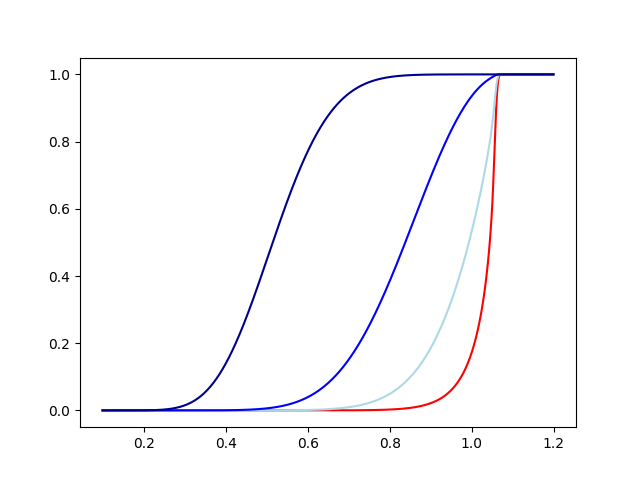
\includegraphics[width=.6\textwidth]{./Figures/H0_H1_comparison.png}\hfill
	\caption{Comparison of $F_R^0(r)$ (red) and three different versions of $F_R^1(r)$ corresponding to $|\mu_A - \mu_B| = 0.5, 1, 2$ (lightblue, blue, darkblue).}
	\label{fig:H0_H1}
\end{figure}

The next result shows large sample size properties of $R$.
\begin{lemma}[Large sample size]\label{lem:large_sample}
	Let $n \to \infty$ and assume that $n_{A} /n \to a \in (0, 1)$, $n_B/n \to 1 - a$. Then, under $H_0$, $R$ converges to $1$ in probability.
\end{lemma}
This is in line with the results in Figure \ref{fig:F_R}.

\begin{figure}[H]
	\centering
	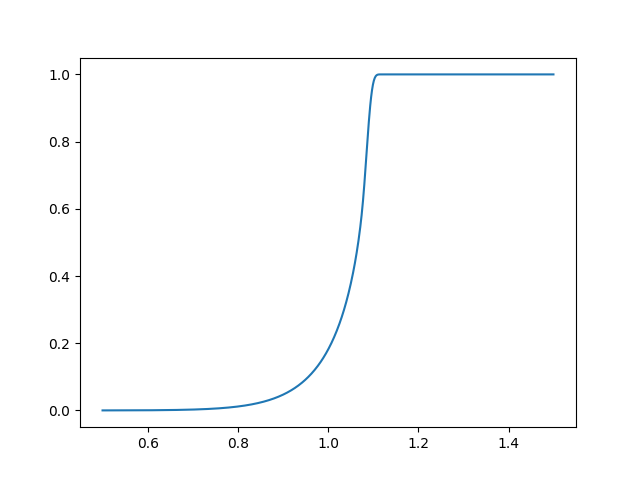
\includegraphics[width=.5\textwidth]{./Figures/10_13_F_R.png}\hfill
	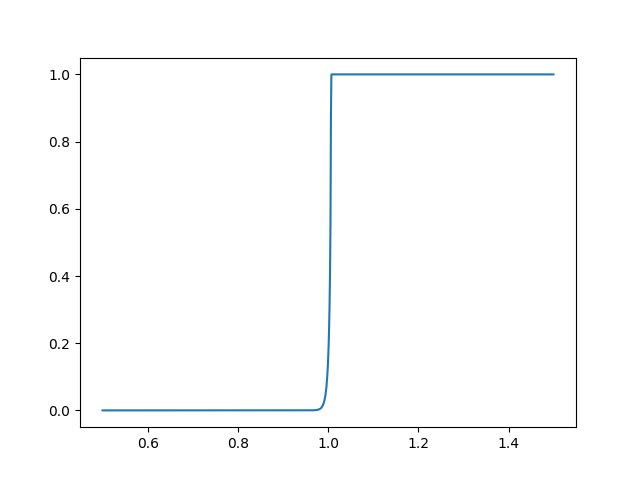
\includegraphics[width=.5\textwidth]{./Figures/160_170_F_R.png}\hfill
	\caption{$F_R^0(r)$ for $(n_A, n_B) = (10, 13)$ and $(n_A, n_B) = (160, 170)$.}
	\label{fig:F_R}
\end{figure}

%Figure \ref{fig:F_R_2} shows how the distributions change when $n_A, n_B$ vary while $n$ is fixed. It seems that low quantiles are not much affected by unbalancedness of $(n_A, n_B)$.
%
%\begin{figure}[H]
%	\centering
%	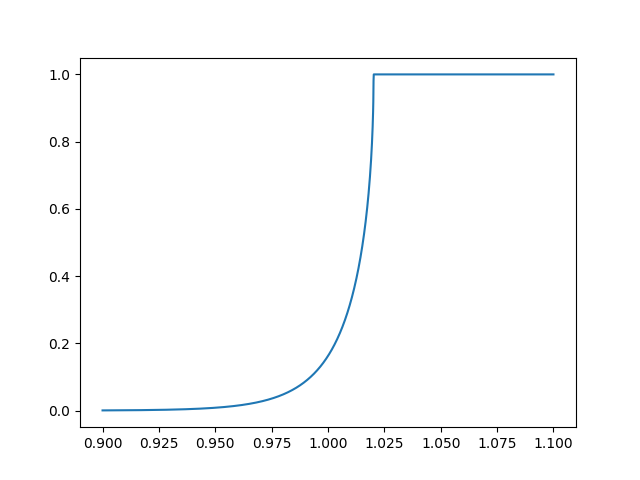
\includegraphics[width=.5\textwidth]{./Figures/50_50_F_R.png}\hfill
%	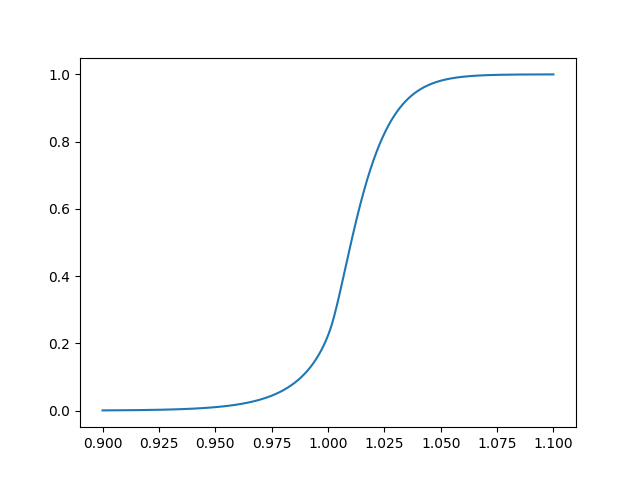
\includegraphics[width=.5\textwidth]{./Figures/95_5_F_R.png}\hfill
%	\caption{$F_R^0(r)$ for $(n_A, n_B) = (50, 50)$ and $(n_A, n_B) = (95, 5)$.}
%	\label{fig:F_R_2}
%\end{figure}




\section{The stopping rule}

\section{Numerical illustration}

\section{Appendix: Proofs}

\begin{proof}[Proof of Lemma \ref{lem:MSEP_0}]
	Since $\hat \mu_0$ is constant is on $D_j$, we have
	\begin{align*}
		\MSEP_j^0  = & \E\left[ (Y^* - \mu_{D_j})^2 \mid X^* \in D_j,  n_{D_j} \right]
		+ \E \left[ (\mu_{D_j} - \hat\mu_0(X^*))^2 \mid X^* \in D_j, n_{D_j} \right]                                                                           \\
		             & \quad + 2\E \left[ (Y^* - \mu_{D_j})( \mu_{D_j} - \widehat \mu_0(X^*)) \mid X^* \in D_j,  n_{D_j}  \right]                              \\
		=            & \sigma_{D_j}^2 +
		\E \left[ \left(\left(\frac{1}{n_{D_j}}\sum_{i =1}^{n_{D_j}} Y_i \right) - \mu_{D_j}  \right)^2 \mid  n_{D_j}, X_1, \dots, X_{n_{D_j}} \in D_j \right] \\
		=            & \sigma_{D_j}^2 +
		\frac{1}{n_{D_j}^2}\E \left[ \left(\sum_{i =1}^{n_{D_j}} (Y_i - \mu_{D_j}) \right)^2 \mid  n_{D_j}, X_1, \dots, X_{n_{D_j}} \in D_j  \right]           \\
		=            & \sigma_{D_j}^2 +
		\frac{1}{n_{D_j}^2}\sum_{i =1}^{n_{D_j}} \E \left[(Y_i - \mu_{D_j})^2 \mid X_i \in D_j \right]                                                         \\
		=            & \sigma_{{D_j}}^2\left(1 + \frac{1}{n_{D_j}} \right).
	\end{align*}
	In the second equality, the mixed term vanishes since, given $X^* \in D_j$, $\hat \mu_0(X^*, (X_i, Y_i)_{i=1}^N) = \hat \mu_0((X_i, Y_i)_{i=1}^N)$ only depends on trainings data and is hence independent of $Y^*$.
\end{proof}

\begin{proof}[Proof of Lemma \ref{lem:MSEP1}]
	Conditioning yields
	\begin{align*}
		\MSEP^1_j
		= & \E \left[
		\left(Y^* - \hat \mu_1(X^*)\right)^2 \mid X^* \in A_j, n_{A_j} \right] \P(X^* \in A_j \mid X^* \in D_j )                                           \\
		+ & \E \left[
			\left(Y^* - \hat \mu_1(X^*)\right)^2 \mid X^* \in B_j,  n_{B_j}
		\right] \P(X^* \in B_j \mid X^* \in D_j )                                                                                                          \\
		= & \sigma_{{A_j}}^2\left(1 + \frac{1}{n_{A_j}} \right)\pi_{A_j \mid D_j} + \sigma_{{B_j}}^2\left(1 + \frac{1}{n_{B_j}} \right)\pi_{B_j \mid D_j},
	\end{align*}
	where, in the last equality, we have applied Lemma \ref{lem:MSEP_0} and the fact that $\hat \mu_1$ is constant on $A_j$ and on $B_j$.
\end{proof}

\begin{proof}[Proof of Lemma \ref{lem:distr_R}]
	Assume without loss of generality that $X_1, \dots, X_{n_A} \in A$ and $X_{n_A + 1}, \dots, X_n \in B$. We wish to determine the distribution function $F_R^0$ of
	$$
		R = \frac{
			\frac{n_A + 1}{n_A - 1} \sum_{i=1}^{n_A} (Y_i - \overline Y_A)^2 + \frac{n_B + 1}{n_B - 1} \sum_{i= n_A + 1}^{n} (Y_i - \overline Y_B)^2
		}{
			\frac{n+1}{n -1} \sum_{i=1}^{n} (Y_i - \overline Y)^2
		}
	$$
	under $H_0$, i.e. given that $\mu_A = \mu_B = \mu_D$. For this purpose, we note that for each $r > 0$,
	\begin{align*}
		F_R^0(r) = \P_0(R \leq r) = \P_0(Z_r \leq 0),
	\end{align*}
	where
	\begin{align}\label{eq:Z_r}
		Z_r = \frac{n_A + 1}{n_A - 1} \sum_{i=1}^{n_A} (Y_i - \overline Y_A)^2 + \frac{n_B + 1}{n_B - 1} \sum_{i= n_A + 1}^{n} (Y_i - \overline Y_B)^2 - r
		\frac{n+1}{n -1} \sum_{i=1}^{n} (Y_i - \overline Y)^2.
	\end{align}
	Let
	\begin{align}
		D_A =\left[\begin{array}{@{}c|c@{}}
				           \begin{matrix}
					1 & \cdots & 1 \\
					  & \vdots     \\
					1 & \cdots & 1
				\end{matrix}
				                    & \quad \bigzero \quad \\
				           \hline                          \\
				           \bigzero &
				           \bigzero                        \\
				           \quad
			           \end{array}\right],
		\quad
		I_A =\left[\begin{array}{@{}c|c@{}}
				           \quad                           \\
				           \quad \bigone_{n_A} \quad
				                    & \quad \bigzero \quad \\
				           \quad                           \\
				           \hline                          \\
				           \bigzero &
				           \bigzero                        \\
				           \quad
			           \end{array}\right]
	\end{align}
	and $D_B, I_B$ defined correspondingly, with the one-matrix and the identity matrix in the lower right block instead. We can then rewrite \eqref{eq:Z_r} as a quadratic form
	\begin{align*}
		Z_r = Y^T Q_r Y,
	\end{align*}
	where
	\begin{align*}
		Q_r = & \frac{n_A +1}{n_A -1} \left(I_A - \frac{1}{n_A} D_A\right)^T\left(I_A - \frac{1}{n_A} D_A\right) +        \\
		      & \frac{n_B +1}{n_B -1} \left(I_B - \frac{1}{n_B} D_B\right)^T\left(I_B - \frac{1}{n_B} D_B\right) -        \\
		      & r\frac{n +1}{n -1} \left(I_n - \frac{1}{n} \mathbf{1} \right)^T\left(I_n - \frac{1}{n} \mathbf{1}\right).
	\end{align*}
	Here, $\mathbf{1}$ is the matrix of ones only. Using that all matrices in brackets are symmetric and idempotent,
	\begin{align*}
		 & Q_r = \frac{n_A +1}{n_A -1} \left(I_A - \frac{1}{n_A} D_A\right) +
		\frac{n_B +1}{n_B -1}\left(I_B - \frac{1}{n_B} D_B\right) -
		r\frac{n +1}{n -1}\left(I_n - \frac{1}{n} \mathbf{1}\right) =         \\
		 &
		\left[\begin{array}{@{}c|c@{}}
				      \begin{matrix}
					\frac{n_A +1}{n_A} - \frac{r(n+1)}{n}              & \frac{r(n+1)}{(n-1)n} - \frac{n_A +1}{(n_A -1)n_A} & \cdots \\
					\frac{r(n+1)}{(n-1)n} - \frac{n_A +1}{(n_A -1)n_A} &                                                             \\
					\vdots                                             & \ddots                                             &
				\end{matrix}
				                                          & \begin{matrix}
					                                      \frac{r(n+1)}{(n-1)n} & \cdots & \\
					                                      \vdots                           \\
				                                      \end{matrix}                                           \\
				      \hline                                                                                                           \\
				      \begin{matrix}
					\frac{r(n+1)}{(n-1)n} & \cdots & \\
					\vdots                           \\
				\end{matrix} &
				      \begin{matrix}
					\frac{n_B +1}{n_B} - \frac{r(n+1)}{n}              & \frac{r(n+1)}{(n-1)n} - \frac{n_B +1}{(n_B -1)n_B} & \cdots \\
					\frac{r(n+1)}{(n-1)n} - \frac{n_B +1}{(n_B -1)n_B} &                                                             \\
					\vdots                                             & \ddots                                             &
				\end{matrix} \\
			      \end{array}\right].
	\end{align*}
	$Q_r$ has four distinct eigenvalues
	\begin{align*}
		\lambda_A^r =            & \frac{n_A +1}{n_A -1} - r\frac{n+1}{n-1}, \\
		\lambda_B^r =            & \frac{n_B +1}{n_B -1} - r\frac{n+1}{n-1}, \\
		\lambda_{\text{neg}}^r = & -r\frac{n+1}{n-1},                        \\
		\lambda_0^r =            & 0
	\end{align*}
	with corresponding eigenspaces
	\begin{align}
		\begin{split}\label{eq:Eigenspaces}
			\text{Eig}_{\lambda_A} = &\text{span}\left(
			\begin{bmatrix}
					1      \\
					-1     \\
					0      \\
					\vdots \\
					0      \\
					\mathbf{0}_{n_B}
				\end{bmatrix},
			\dots,
			\begin{bmatrix}
					1      \\
					0      \\
					\vdots \\
					0      \\
					-1     \\
					\mathbf{0}_{n_B}
				\end{bmatrix}
			\right),
			\quad
			\text{Eig}_{\lambda_B} = \text{span}\left(
			\begin{bmatrix}
					\mathbf{0}_{n_A} \\
					1                \\
					-1               \\
					0                \\
					\vdots           \\
					0
				\end{bmatrix},
			\dots,
			\begin{bmatrix}
					\mathbf{0}_{n_{A}} \\
					1                  \\
					0                  \\
					\vdots             \\
					0                  \\
					-1
				\end{bmatrix}
			\right),  \\
			\text{Eig}_{\lambda_{\text{neg}}} = &\text{span}\left(
			\begin{bmatrix}
					n_B    \\
					\vdots \\
					n_B    \\
					-n_A   \\
					\vdots \\
					-n_A
				\end{bmatrix}
			\right), \quad
			\text{Eig}_{\lambda_0} = \text{span}\left(
			\begin{bmatrix}
					1      \\
					\vdots \\
					1
				\end{bmatrix}
			\right)
		\end{split}
	\end{align}
	and hence geometric multiplicities $n_A -1, n_B -1, 1$ and $1$, respectively. Let
	$$
		P = \left[\begin{array}{@{}c|c|c|c@{}}
				P_{11}
				         & \bigzero
				         & \begin{matrix}
					           n_B/\sqrt{n_A^2 n_B + n_A n_B^2} \\
					           \vdots                           \\
					           n_B/\sqrt{n_A^2 n_B + n_A n_B^2}
				           \end{matrix}
				         &
				\begin{matrix}
					1/\sqrt{n} \\
					\vdots     \\
					1/\sqrt{n}
				\end{matrix}                                \\
				\hline
				\bigzero &
				P_{22}
				         & \begin{matrix}
					           -n_A/\sqrt{n_A^2 n_B + n_A n_B^2} \\
					           \vdots                            \\
					           -n_A/\sqrt{n_A^2 n_B + n_A n_B^2}
				           \end{matrix}
				         & \begin{matrix}
					           1/\sqrt{n} \\
					           \vdots     \\
					           1/\sqrt{n}
				           \end{matrix}
			\end{array}\right],
	$$
	where $P_{11}$ ($P_{22}$) is an $n_A \times n_A -1$ ($n_B \times n_B -1$) matrix obtained by applying the Gram-Schmidt orthogonalization to the first $n_A$ (last $n_B$) components of the vectors spanning $\text{Eig}_{\lambda_A}$ ($\text{Eig}_{\lambda_B}$) from \eqref{eq:Eigenspaces} above.

	By Mathai, Provost, "Quadratic forms in random variables", page 29, formula (3.1a.4), it follows that
	\begin{align}
		\begin{split}\label{eq:Z_law}
			Z_r = &Y^T Q_r Y \\
			\eqdis &\sigma^2 \left(
			\lambda_A^r \sum_{i=1}^{n_A - 1} (U_i + b_i)^2
			+ \lambda_B^r \sum_{i= n_A}^{n -2} (U_i + b_i)^2
			+ \lambda_{\text{neg}}^r (U_{n-1} + b_{n-1})^2
			\right).
			%\\
			%\eqdis &\frac{\sigma^2}{n-1} \left( 
			%\frac{2 n_B}{n_A -1} \chi^2_A(n_A -1, \xi_A)
			%+ \frac{2 n_A}{n_B -1} \chi^2_B(n_B -1, \xi_B)
			%- (n+1) \chi^2(1, b_{n-1}^2)
			%\right)
		\end{split}
	\end{align}
	Here, $U_1, \dots, U_{n-1}$ are iid standard normally distributed and, with
	$$
		\bar \mu^T = (\bar \mu_A^T, \bar \mu_B^T) =  \left(\mu_A, \dots, \mu_A, \mu_B, \dots, \mu_B\right) \in \R^{n_A} \times \R^{n_B},
	$$
	$$
		b = \frac{1}{\sigma}P^T \bar \mu =
		\frac{1}{\sigma}\begin{bmatrix}
			P_{11}^T \bar \mu_A                                                                                           \\
			P_{22}^T \bar \mu_B                                                                                           \\
			\left(n_B \sum_{i=1}^{n_A} \bar \mu_i - n_A \sum_{i=n_A + 1}^n \bar \mu_i\right)/\sqrt{n_A^2 n_B + n_A n_B^2} \\
			\left(\sum_{i=1}^n \bar \mu_i \right)/\sqrt{n}
		\end{bmatrix}.
	$$
	\paragraph{Non-central Chi-square}
	Let $X_1, \dots, X_m$ independent normally distributed random variables with means $a_1, \dots, a_m$ and unit variances and set $\xi = \sum_{i=1}^m a_i^2$ (non-centrality parameter). Then, $\sum_{i = 1}^m X_i^2$ follows a non-central chi-squared distribution with $m$ degrees of freedom and is denoted by $\chi^2_m(\xi)$.

	We would like to express \eqref{eq:Z_law} in terms of a linear combination of independent non-central chi-squares. For this purpose, we compute
	$$
		\xi_A = \sum_{i=1}^{n_A -1} b_i^2, \quad \xi_B = \sum_{i=n_A}^{n-2} b_i^2, \text{ and } \quad \xi_{\text{neg}} = b_{n-1}^2.
	$$
	Denote by $\tilde P_{11}^T$ the orthogonal $n_A \times n_A$ matrix obtained by adding $(1/\sqrt{n_A}, \dots, 1/\sqrt{n_A}) \in \R^{n_A}$  as an additional row to $P_{11}^T$. We then get
	\begin{align*}
		\xi_A  = \sum_{i=1}^{n_A -1} b_i^2 =
		  & \frac{1}{\sigma^2} \left(\sum_{i=1}^{n_A} \left(\left(\tilde P_{11}^T \bar \mu_A \right)_i \right)^2 - |(1/\sqrt{n_A}, \dots, 1/\sqrt{n_A}) \bar\mu_A|^2 \right) \\
		= & \frac{1}{\sigma^2} \left(\sum_{i=1}^{n_A} \bar \mu_i^2 - \frac{1}{n_A} \left(\sum_{i=1}^{n_A} \bar \mu_i \right)^2 \right)
		= \frac{1}{\sigma^2} \left(n_A \mu_A^2 - n_A \mu_A^2 \right) = 0,
	\end{align*}
	where we have used the orthogonality of $\tilde P_{11}$ in the third equality. Similarly, one gets
	$$
		\xi_B = \frac{1}{\sigma^2} \left(n_B \mu_B^2 - n_B \mu_B^2 \right) = 0
	$$
	and
	$$
		\xi_{\text{neg}} = \frac{\left(n_B \sum_{i=1}^{n_A} \bar \mu_i - n_A \sum_{i=n_A + 1}^n \bar \mu_i \right)^2}{\sigma^2\left(n_A^2 n_B + n_A n_B^2\right)} =
		\frac{n_A n_B (\mu_A - \mu_B)^2}{n\sigma^2}.
	$$
	Altogether, we can rewrite \eqref{eq:Z_law} to get
	\begin{align}\label{eq:Z_law2}
		Z_r \eqdis
		 & \sigma^2 \left(
		\lambda_{A}^r \chi^2_{n_A -1}
		+ \lambda_{B}^r \tilde \chi^2_{n_B -1}
		+ \lambda_{\text{neg}}^r \bar \chi_1^2(\xi_{\text{neg}})
		\right),
	\end{align}
	where $\chi^2_{n_A -1}, \tilde \chi^2_{n_B -1}$ and $\bar \chi_1^2(\xi_{\text{neg}})$ are independent.

	Under $H_0$, we have $\mu_A = \mu_B$, which implies that $\xi_{\text{neg}} = 0$. It then follows that
	\begin{align}\label{eq:Z_law3}
		Z_r \eqdis
		 & \sigma^2 \left(
		\lambda_{A}^r \chi^2_{n_A -1}
		+ \lambda_{B}^r \tilde \chi^2_{n_B -1}
		+ \lambda_{\text{neg}}^r \bar \chi_1^2
		\right),
	\end{align}
	where all chi-squares are central and independent. Denoting the random variable in brackets by $Z_r^1$, this means that
	$$
		F_R^0(r) = \P_0(Z_r \leq 0) = \P_0(Z_r^1 \leq 0).
	$$


\end{proof}

\begin{proof}[Proof of Lemma \ref{lem:large_sample}]
	Let $n \to \infty$ and assume that $n_A /n \to a \in (0, 1)$, $n_B/n \to 1 - a$. We first want to investigate the weak limit of $Z_r^1$ under $H_0$, i.e. the limit of
	\begin{align}\label{eq:Z_lim}
		\tilde \lambda_A^r \frac{\chi^2_{n_A - 1}}{n_A - 1} + \tilde \lambda_B^r \frac{\tilde \chi^2_{n_B - 1}}{n_B - 1} + \lambda_{\text{neg}}^r \bar \chi^2_{1},
	\end{align}
	where all chi-squares are independent and
	\begin{align*}
		\tilde \lambda_A^r = & \frac{(n_A + 1)(n-1) - r(n+1)(n_A-1)}{n-1},                                                    \\
		\tilde \lambda_B^r = & \frac{(n_B + 1)(n-1) - r(n+1)(n_B-1)}{n-1}, \quad \lambda_{\text{neg}}^r = -r \frac{n+1}{n-1}.
	\end{align*}
	The first two standardised chi-squares in \eqref{eq:Z_lim} each converge to $1$ in probability. Moreover,
	\begin{align*}
		 & \lambda_{\text{neg}}^r \to - r,                                          \\
		 & \tilde \lambda_A^r = \frac{2 n_B}{n-1} + \frac{(1-r)(n+1)(n_A - 1)}{n-1}
		\to
		\begin{cases}
			2(1-a),   & r=1  \\
			- \infty, & r >1 \\
			+ \infty, & r <1
		\end{cases}
	\end{align*}
	and similarly
	\begin{align*}
		\tilde \lambda_B^r
		\to
		\begin{cases}
			2a,       & r=1   \\
			- \infty, & r >1  \\
			+ \infty, & r <1.
		\end{cases}
	\end{align*}
	Hence, under $H_0$, we get convergence in distribution by the Slutzky Theorem
	\begin{align*}
		Z_r^1 \to Z_r^{1,\infty} :=
		\begin{cases}
			2 - \bar \chi_{1}, & r=1   \\
			- \infty,          & r >1  \\
			+ \infty,          & r <1.
		\end{cases}
	\end{align*}
	Since $Z_{r}^{1,\infty}$ has no mass at $0$ for any $r > 0$, this implies that
	\begin{align*}
		F_R^0(r) = \P_0(Z_r^1 \leq 0) \to \P_0(Z_r^{1, \infty} \leq 0) =
		\begin{cases}
			\P(\bar \chi_{1} \geq 2), & r=1   \\
			1,                        & r >1  \\
			0,                        & r <1.
		\end{cases}
	\end{align*}
	This shows that the ratio $R$ converges to $1$ under $H_0$ in distribution (and hence in probability). Note that the limit does not depend on $a$.

\end{proof}



\begin{thebibliography}{99}

\end{thebibliography}

\end{document}
